\documentclass[a4paper,11pt]{article}
\usepackage[T1]{fontenc}
\usepackage{lmodern}
\usepackage{babel}
\babelprovide[main,import]{spanish}
\usepackage[margin=2.4cm,headheight=14pt]{geometry}
\usepackage{microtype}
\usepackage{graphicx,xcolor,booktabs,array,tabularx,enumitem,float}
\usepackage[font=small,skip=6pt]{caption}
\usepackage{subcaption}
\usepackage{fancyhdr}
\usepackage[hidelinks]{hyperref}

\definecolor{navy}{HTML}{263951}
\definecolor{greytext}{HTML}{475568}
\definecolor{panel}{HTML}{EFF3F7}
\definecolor{marco}{HTML}{C9D2DC}
\definecolor{alerta}{HTML}{B42318}
\definecolor{alertafondo}{HTML}{FDECEA}
\hypersetup{
  pdftitle={SolarBell - Manual de usuario},
  pdfauthor={Andrés Felipe Ortiz Rodríguez, Néstor Junior Hernández López, José Enrique Otero Pineda, Julián Camilo Doria Guevara},
  pdfsubject={Manual de operación del Proyecto de Aula Semestral},
  bookmarksopen=true
}
\addto\captionsspanish{%
  \renewcommand{\contentsname}{Índice}%
  \renewcommand{\figurename}{Figura}%
  \renewcommand{\tablename}{Tabla}%
}
\captionsetup[sub]{font=footnotesize,skip=4pt,justification=centering}
\setcounter{tocdepth}{2}
\setlength{\parskip}{5pt plus 1pt}
\setlength{\parindent}{0pt}
\setlength{\emergencystretch}{2em}
\renewcommand{\arraystretch}{1.19}
\setlist{topsep=3pt,itemsep=4pt,parsep=0pt,leftmargin=*}
\raggedbottom
\newcolumntype{Y}{>{\raggedright\arraybackslash}X}
\newcolumntype{P}[1]{>{\raggedright\arraybackslash}p{#1}}
\newcommand{\pin}[1]{\texttt{#1}}
\newcommand{\boton}[1]{\textbf{#1}}
\newcommand{\nota}[1]{%
  \par\smallskip\noindent{\setlength{\fboxsep}{9pt}%
  \colorbox{panel}{\parbox{\dimexpr\linewidth-2\fboxsep\relax}{\small #1}}}%
  \par\smallskip
}
\newcommand{\alerta}[1]{%
  \par\smallskip\noindent{\setlength{\fboxsep}{9pt}\setlength{\fboxrule}{0.8pt}%
  \fcolorbox{alerta}{alertafondo}{\parbox{\dimexpr\linewidth-2\fboxsep-1.6pt\relax}{\small #1}}}%
  \par\smallskip
}
% Captura de pantalla del teléfono con un marco fino.
\newcommand{\captura}[1]{{\setlength{\fboxsep}{0pt}\setlength{\fboxrule}{0.4pt}%
  \fcolorbox{marco}{white}{\includegraphics[width=\dimexpr\linewidth-0.8pt\relax]{figuras/app/#1}}}}
% \pantalla[ancho]{archivo}{subtítulo}
\newcommand{\pantalla}[3][0.27]{%
  \begin{subfigure}[t]{#1\linewidth}\centering\captura{#2}\caption{#3}\end{subfigure}}
\pagestyle{fancy}
\fancyhf{}
\fancyhead[L]{\small\color{greytext}SolarBell}
\fancyhead[R]{\small\color{greytext}Manual de usuario}
\fancyfoot[C]{\small\thepage}
\renewcommand{\headrulewidth}{0.35pt}

\begin{document}
\begin{titlepage}
  \centering
  \vspace*{1.15cm}
  {\large\bfseries UNIVERSIDAD DE CÓRDOBA\par}
  \vspace{0.24cm}
  {\bfseries FACULTAD DE INGENIERÍA\par}
  \vspace{0.20cm}
  {\bfseries PROGRAMA DE INGENIERÍA DE SISTEMAS\par}
  \vspace{0.20cm}
  {\bfseries SEDE MONTERÍA\par}
  \vfill
  {\large\bfseries PROYECTO DE AULA SEMESTRAL\par}
  \vspace{0.9cm}
  {\Huge\bfseries\color{navy} Manual de usuario\par}
  \vspace{0.25cm}
  {\LARGE\bfseries SolarBell\par}
  \vspace{0.38cm}
  {\large Sistema de timbre automatizado con energía solar\par}
  \vspace{0.7cm}
  {\color{greytext}Instalación documentada\par
  Institución Educativa Cecilia de Lleras, Montería\par}
  \vfill
  {\bfseries Presentado por\par}
  \vspace{0.28cm}
  Andrés Felipe Ortiz Rodríguez\par
  Néstor Junior Hernández López\par
  José Enrique Otero Pineda\par
  Julián Camilo Doria Guevara\par
  \vfill
  {\bfseries Docentes\par}
  \vspace{0.27cm}
  Antonio Fernando Movilla Quintero\par
  Milton Eduardo Hernández Zakzuk\par
  \vfill
  {\bfseries Arquitectura del Computador y Sistemas Operativos\par}
  \vspace{0.28cm}
  Montería, noviembre de 2026\par
  \vspace*{0.2cm}
\end{titlepage}

\pagenumbering{arabic}
\alerta{\textbf{Seguridad.} No abra el gabinete de la campana. Adentro hay una batería, un inversor que entrega 110\,V y la conexión del pulsador de pared a la red eléctrica del colegio. Toda la operación diaria se hace desde el teléfono o con el pulsador instalado. Si algo dentro del gabinete parece dañado, avise a soporte.}

\tableofcontents

% ---------------------------------------------------------------------------
\clearpage
\section{Alcance, acceso y responsabilidades}
\label{sec:alcance}
Este manual explica cómo operar SolarBell desde un teléfono Android. Está dirigido al personal de la Institución Educativa Cecilia de Lleras que administra los avisos de la jornada escolar. Describe la aplicación de la rama \pin{main}, revisión \pin{0adeb14}, con la campana en el firmware 0.8.0 \cite{repo,firmware,informe}.

Cada sección sigue el mismo orden: qué se ve en la pantalla, los pasos para hacer la tarea y cómo comprobar que quedó bien. Las capturas corresponden a esa versión de la aplicación conectada a una campana de prueba que responde igual que el firmware 0.8.0. Los horarios, las fechas, los toques del historial y los nombres de redes de las capturas son ejemplos: en el colegio verá los que haya configurado.

\subsection{Quién puede usar la campana}
SolarBell no tiene usuarios ni contraseña dentro de la aplicación. La única protección es la clave de la red Wi-Fi \textbf{SolarBell} que crea la campana (y, si la campana se unió a la red del colegio, la clave de esa red). Cualquier persona con la aplicación instalada y conectada a esa red puede ver el horario, cambiarlo y hacer sonar la campana \cite{firmware}.

Por eso la clave se entrega solo a las personas autorizadas por el colegio, por el canal que el colegio defina. Si sospecha que alguien no autorizado la conoce, avise a soporte para cambiarla.

\begin{table}[H]
\centering\small
\caption{Responsabilidades de operación}
\begin{tabularx}{\linewidth}{@{}P{4.3cm}Y@{}}
\toprule
\textbf{Responsable} & \textbf{Tarea} \\
\midrule
Operador del timbre & Consulta la agenda, configura los avisos y las fechas especiales autorizados y verifica que suenen. \\
Coordinación del colegio & Define las horas de la jornada, las fechas con cambios y las franjas en que se permiten pruebas sonoras. Autoriza a quién se entrega la clave. \\
Soporte del sistema & Instala la aplicación, entrega la clave de la red SolarBell, cambia la clave si hace falta y atiende fallas de conexión, reloj, batería o accionamiento. Es el único que abre el gabinete. \\
\bottomrule
\end{tabularx}
\end{table}

\nota{\textbf{Para empezar.} Tenga a mano el teléfono con SolarBell instalada, la clave de la red y el horario aprobado por coordinación. Haga las pruebas sonoras en una franja acordada con el colegio.}

% ---------------------------------------------------------------------------
\clearpage
\section{Conozca la aplicación}
\label{sec:navegacion}
\subsection{Las seis pestañas}
La barra de la parte inferior tiene seis pestañas. La pestaña abierta aparece resaltada. Elija la pestaña según la tarea \cite{repo}.

\begin{table}[H]
\centering\small
\caption{Qué se hace en cada pestaña}
\begin{tabularx}{\linewidth}{@{}P{2.4cm}Y P{2.6cm}@{}}
\toprule
\textbf{Pestaña} & \textbf{Qué puede hacer} & \textbf{Dónde se explica} \\
\midrule
Inicio & Ver la fecha, la cuenta regresiva al próximo aviso y el resumen del día. & Sección~\ref{sec:inicio} \\
Horario & Ver los días con timbrado y crear, editar o eliminar los avisos de la semana. & Sección~\ref{sec:horario} \\
Tocar & Hacer sonar la campana en el momento, seguir el toque en curso y detenerlo. & Sección~\ref{sec:tocar} \\
Fechas & Crear, editar o eliminar un horario distinto para un día concreto, o dejar un día sin campana. & Sección~\ref{sec:fecha} \\
Historial & Consultar los toques que ya sonaron, buscarlos por nombre o por fecha, ver cómo sonó cada uno y borrar registros. & Sección~\ref{sec:historial} \\
Campana & Ver si la campana está conectada y en hora, unirla al Wi-Fi del colegio y cambiar la apariencia. & Sección~\ref{sec:conexion} \\
\bottomrule
\end{tabularx}
\end{table}

\subsection{Controles que se repiten}
Estos controles aparecen en varias pantallas y funcionan igual en todas:

\begin{itemize}
  \item \textbf{Hojas.} Los formularios se abren como una hoja que sube desde abajo, con el título arriba y el botón principal al final. La \textbf{X} de la esquina cierra la hoja sin guardar.
  \item \textbf{Botones $-$ y $+$.} Ajustan un número (toques o segundos). También puede tocar el número y escribirlo; se aplica al salir del campo. Los botones rojos son los de las pausas.
  \item \textbf{Papelera.} Al tocarla aparece una ventana que pregunta, por ejemplo, \textbf{¿Eliminar timbrado?} y dice qué se va a quitar. \boton{Eliminar} borra; \boton{Cancelar} cierra la ventana sin borrar nada. Lo eliminado no se puede recuperar.
  \item \textbf{Avisos.} Después de guardar aparece arriba un aviso corto, por ejemplo \textbf{Timbrado agregado}. Un aviso con una \textbf{X} roja indica que la campana no recibió el cambio.
  \item \textbf{Guardado.} No hay botón de sincronizar. Cada cambio confirmado se envía a la campana en ese momento. Si la campana no responde, la aplicación vuelve al último horario que la campana confirmó.
\end{itemize}

\subsection{Pantalla de Inicio}
\label{sec:inicio}
Inicio es la primera pantalla al abrir la aplicación. Sirve para saber, de un vistazo, qué va a sonar y cuándo.

\begin{figure}[H]
\centering
\pantalla{inicio}{Día normal: faltan 9 min 58 s para el Descanso.}\hfill
\pantalla{inicio-especial}{Fecha especial: el aviso viene de «Izada de bandera».}\hfill
\pantalla{inicio-sin-timbrados}{Sábado: el día no está en el horario habitual.}
\caption{Tres casos de la pantalla de Inicio}
\label{fig:inicio}
\end{figure}

\begin{enumerate}
  \item Arriba están \textbf{Hoy} y la fecha. Si debajo aparece en rojo \textbf{Campana fuera de alcance}, el teléfono no se está comunicando con la campana; tóquelo para ir a \textbf{Campana} (sección~\ref{sec:estado}).
  \item \textbf{Cuenta regresiva} muestra el tiempo que falta para el próximo aviso. Debajo, en una franja, están el nombre y la hora de ese aviso. La línea de la franja se llena a medida que se acerca la hora.
  \item Si el próximo aviso pertenece a una fecha especial, aparece debajo \textbf{Fecha especial:} y su nombre (Figura~\ref{fig:inicio}, centro).
  \item En el resumen, \textbf{Hoy} cuenta los avisos previstos para el día, \textbf{Restantes} los que aún no han sonado y \textbf{Especiales} las fechas especiales de hoy en adelante.
  \item La línea de tiempo marca cada aviso del día: gris los que ya pasaron, azul el próximo y rojo los que faltan. El punto azul es la hora actual. Debajo se repite el \textbf{Próximo timbrado}.
\end{enumerate}

Cuando el día no tiene avisos, el resumen lo explica con una frase: «Sábado no está en el horario habitual», «Acto cívico: la campana no suena hoy» o «Acto cívico no tiene timbrados». La cuenta regresiva sigue mostrando el próximo aviso de otro día (Figura~\ref{fig:inicio}, derecha). Si no hay ningún aviso guardado, la cuenta regresiva dice \textbf{Sin timbrados} y ofrece el botón \textbf{Configurar horario}.

\nota{El horario, las fechas especiales y el historial viven en la campana, no en el teléfono. La campana sigue sonando con lo guardado aunque el teléfono se vaya, siempre que tenga energía y el reloj esté en hora \cite{firmware}.}

% ---------------------------------------------------------------------------
\clearpage
\section{Instalación y conexión}
\label{sec:conexion}
\subsection{Instalar y abrir la aplicación}
\begin{enumerate}
  \item Pida a soporte el instalador APK de SolarBell. La aplicación funciona desde Android 7.0 \cite{apk}.
  \item Abra el archivo y siga las indicaciones de Android. Si el teléfono es del colegio y la instalación aparece bloqueada, pida a soporte que la haga.
  \item Abra \textbf{SolarBell} desde la lista de aplicaciones. Abre directamente en \textbf{Inicio}, sin pedir usuario ni contraseña.
\end{enumerate}

\subsection{Primera conexión a la red SolarBell}
\label{sec:primera}
\begin{enumerate}
  \item Acérquese a la campana. La red llega a unos metros del gabinete.
  \item En los ajustes de Wi-Fi de Android, elija la red \textbf{SolarBell} y escriba la clave que le entregó soporte.
  \item Android puede avisar que la red no tiene Internet. Elija \textbf{seguir conectado}: la aplicación no usa Internet, habla directamente con la campana.
  \item Revise que la fecha, la hora y la zona horaria del teléfono sean correctas. Al conectarse, la aplicación pone la campana en la hora del teléfono si difieren en más de 5 segundos.
  \item Abra SolarBell y vaya a \textbf{Campana}. Espere a ver \textbf{Conectada} y \textbf{En hora} (Figura~\ref{fig:estado}, izquierda).
  \item Vuelva a \textbf{Inicio} y confirme que la fecha y el próximo aviso coinciden con el horario del colegio.
\end{enumerate}

\begin{figure}[H]
\centering
\pantalla{campana}{Conectada y en hora.}\hspace{1.2cm}
\pantalla{campana-fuera}{Fuera de alcance: no hay datos de reloj ni firmware.}
\caption{Tarjeta de estado en la pestaña Campana}
\label{fig:estado}
\end{figure}

\begin{table}[H]
\centering\small
\caption{Qué red usar}
\begin{tabularx}{\linewidth}{@{}P{4.2cm}Y@{}}
\toprule
\textbf{Red} & \textbf{Cuándo usarla} \\
\midrule
Red propia \textbf{SolarBell} & Primera conexión, unir la campana a la red del colegio o recuperar el acceso cerca del gabinete. Está disponible mientras el interruptor del Wi-Fi esté en su posición normal (sección~\ref{sec:interruptor}). \\
Red del colegio & Operación diaria desde otro punto del colegio, cuando la campana ya se unió a esa red (sección~\ref{sec:redcolegio}). Es la única red disponible si soporte dejó la campana en modo de ahorro. \\
\bottomrule
\end{tabularx}
\end{table}

\subsection{Unir la campana al Wi-Fi del colegio}
\label{sec:redcolegio}
Esta opción permite operar la campana desde la red del colegio sin acercarse al gabinete. En la aplicación aparece en \textbf{Campana} con el título \textbf{Wi-Fi de casa}; ese nombre también se usa para la red del colegio. Necesita la autorización del colegio, el nombre de una red de \textbf{2,4\,GHz} y su clave \cite{repo,firmware}.

\begin{enumerate}
  \item Conecte el teléfono a la red \textbf{SolarBell} y abra \textbf{Campana}. Espere \textbf{Conectada}.
  \item En la tarjeta \textbf{Wi-Fi de casa}, pulse \boton{Elegir red} (o \boton{Cambiar red} si ya hay una guardada).
  \item Se abre la hoja \textbf{Wi-Fi de la campana} y la campana busca redes (\textbf{Buscando…}). Cuando termina, aparece la lista \textbf{Redes cercanas} con la intensidad de la señal y un candado en las que piden clave (Figura~\ref{fig:wifi1}). Si no aparece la red, pulse \boton{Buscar de nuevo}.
  \item Toque la red. En la ventana que se abre escriba la clave (de 8 a 63 caracteres). El ojo de la derecha muestra u oculta lo escrito para revisarlo.
  \item Pulse \boton{Conectar}. El botón cambia a \textbf{Uniéndose…}. Puede tardar hasta medio minuto y el teléfono puede perder la red SolarBell un momento: es normal (Figura~\ref{fig:wifi2}).
  \item Si la unión funciona, aparece el aviso \textbf{Campana unida a …} con la dirección IP que le dio la red, y la tarjeta queda en \textbf{Unida a «nombre de la red» · IP}.
  \item Ya puede conectar el teléfono a la red del colegio. La aplicación encuentra la campana sola en esa red.
\end{enumerate}

\begin{figure}[H]
\centering
\pantalla{campana-wifi-buscando}{La campana busca redes.}\hfill
\pantalla{campana-wifi-redes}{Redes cercanas.}\hfill
\pantalla{campana-wifi-clave}{Clave escrita y visible con el ojo.}
\caption{Elegir la red del colegio}
\label{fig:wifi1}
\end{figure}

\begin{figure}[H]
\centering
\pantalla{campana-wifi-uniendose}{Esperando a que se una.}\hfill
\pantalla{campana-wifi-fallo}{Clave incorrecta: corrija y vuelva a conectar.}\hfill
\pantalla{campana-wifi-unida}{Unida, con la IP asignada.}
\caption{Resultado de la unión}
\label{fig:wifi2}
\end{figure}

\paragraph{Si no se une.} La ventana muestra en rojo el motivo y la campana vuelve a la red que tenía antes. Los motivos más comunes son:

\begin{table}[H]
\centering\small
\caption{Mensajes al unir la campana a una red}
\label{tab:wifi}
\begin{tabularx}{\linewidth}{@{}P{6.2cm}Y@{}}
\toprule
\textbf{Mensaje} & \textbf{Qué hacer} \\
\midrule
Clave incorrecta & Revise mayúsculas y números con el ojo y vuelva a pulsar \boton{Conectar}. \\
No se encontró la red (¿está lejos o es de 5\,GHz?) & Elija una red de 2,4\,GHz o pida a soporte que revise el alcance. \\
La señal de la red es muy débil & El punto de acceso está lejos del gabinete. Avise a soporte. \\
Se unió a la red, pero no recibió dirección IP & La red del colegio no le asignó dirección. Consulte con quien administra esa red. \\
La campana no contestó. Revisa que sigas en su red… & El teléfono salió de la red SolarBell. Vuelva a conectarse a ella y revise la tarjeta. \\
\bottomrule
\end{tabularx}
\end{table}

\begin{figure}[H]
\centering
\pantalla{campana-wifi-oculta}{Red oculta: nombre y clave a mano.}\hspace{1.2cm}
\pantalla{campana-wifi-olvidada}{Tras \textbf{Olvidar}: Sin red guardada.}
\caption{Red oculta y olvidar la red guardada}
\label{fig:wifi3}
\end{figure}

\paragraph{Red oculta.} Si la red del colegio no se anuncia, pulse \boton{Escribir el nombre a mano (red oculta)} al final de la lista, escriba el nombre exacto y la clave, y pulse \boton{Conectar}.

\paragraph{Olvidar la red.} Conectado a \textbf{SolarBell}, pulse \boton{Olvidar} en la tarjeta. Aparece el aviso \textbf{Red olvidada} y la tarjeta vuelve a \textbf{Sin red guardada}. Desde ese momento la campana solo se alcanza por su red propia.

\subsection{Estado de la campana y cómo recuperarla}
\label{sec:estado}
Abra \textbf{Campana} cuando necesite confirmar el enlace, comprobar la hora o reportar la versión instalada \cite{repo}.

\begin{figure}[H]
\centering
\pantalla[0.25]{campana-completa}{Pestaña Campana completa.}
\caption{De arriba abajo: estado, cómo conectarse, Wi-Fi de casa y apariencia}
\label{fig:campana}
\end{figure}

\begin{table}[H]
\centering\small
\caption{Cómo leer la tarjeta de estado}
\begin{tabularx}{\linewidth}{@{}P{2.3cm}P{4.4cm}Y@{}}
\toprule
\textbf{Campo} & \textbf{Lectura normal} & \textbf{Si dice otra cosa} \\
\midrule
Estado & \textbf{Conectada} (punto azul) & \textbf{Buscando…}: espere unos segundos. \textbf{Fuera de alcance, vista hace…} (punto rojo): el teléfono no llega a la campana; vea la sección~\ref{sec:diagnostico}. \\
Reloj & \textbf{En hora} & \textbf{Sin hora}: la campana perdió la hora y no tocará el horario. Revise la hora del teléfono y vuelva a abrir la aplicación conectado a la campana. \\
Firmware & \textbf{0.8.0} & Otro número indica otra versión de la campana. Con el enlace caído aparece una raya. \\
\bottomrule
\end{tabularx}
\end{table}

\paragraph{Búsqueda automática.} No hace falta escribir ninguna dirección. La aplicación busca la campana sola, en su red propia o en la red del colegio, y la vuelve a buscar cada cierto tiempo si cambió de red. Para buscarla al momento, pulse \boton{Buscar campana} en la tarjeta \textbf{Wi-Fi de casa}; el botón está siempre, aunque la campana esté fuera de alcance. Espere el aviso \textbf{Campana encontrada}. Si dice \textbf{No se encontró la campana}, conéctese a la red \textbf{SolarBell} cerca del gabinete e intente de nuevo.

\paragraph{Apariencia.} Al final de \textbf{Campana}, elija \boton{Claro} u \boton{Oscuro}. El cambio solo afecta a este teléfono (Figura~\ref{fig:oscuro}).

\begin{figure}[H]
\centering
\pantalla{inicio-oscuro}{Inicio.}\hfill
\pantalla{horario-oscuro}{Horario.}\hfill
\pantalla{campana-oscuro}{Campana, con el selector de apariencia.}
\caption{Apariencia oscura}
\label{fig:oscuro}
\end{figure}

% ---------------------------------------------------------------------------
\clearpage
\section{Horario habitual}
\label{sec:horario}
El horario habitual es la lista de avisos que suenan cada día de clase. En la aplicación cada aviso se llama \emph{timbrado} y tiene un nombre, una hora y un patrón de toques.

\subsection{Consultar el horario}
Abra \textbf{Horario}. Arriba, \textbf{Días con timbrado} muestra en rojo los días en que suena el horario (en el colegio, \textbf{Lunes a viernes}). Debajo está la lista \textbf{Timbrados}, ordenada por hora, con el número total a la derecha. Cada fila muestra la hora, el nombre y un resumen del patrón, por ejemplo «2 toques de 1,5\,s» \cite{repo}.

\begin{figure}[H]
\centering
\pantalla{horario}{Parte superior de la lista.}\hspace{1.2cm}
\pantalla{horario-completo}{Lista completa y botón \textbf{Agregar timbrado}.}
\caption{Pestaña Horario con el horario del colegio}
\label{fig:horario}
\end{figure}

\nota{\textbf{Los círculos de los días son solo de consulta.} En esta versión no se cambian desde la aplicación. Para que un día de clase no suene o suene distinto (un festivo, un acto cívico, una jornada pedagógica), use \textbf{Fechas} (sección~\ref{sec:fecha}).}

\subsection{Agregar un timbrado}
\begin{enumerate}
  \item En \textbf{Horario}, baje hasta el final de la lista y pulse \boton{Agregar timbrado}. Se abre la hoja \textbf{Nuevo timbrado} con una hora sugerida (una hora después del último aviso).
  \item Escriba el \textbf{Nombre del timbrado}, por ejemplo «Entrada» o «Fin del descanso». Si lo deja vacío, la lista lo mostrará como «Timbrado».
  \item Toque \textbf{Hora en que suena} y elija la hora.
  \item Ajuste \textbf{Veces que suena}, \textbf{Duración por toque} y \textbf{Pausa entre toques} (sección~\ref{sec:patron}). Debajo, \textbf{Patrón} dibuja los toques y suma el tiempo total.
  \item Pulse \boton{Agregar timbrado} al final de la hoja. Aparece el aviso \textbf{Timbrado agregado} y el nuevo aviso queda en su lugar según la hora.
\end{enumerate}

\begin{figure}[H]
\centering
\pantalla{horario-nuevo-vacio}{Hoja vacía, con la hora sugerida.}\hfill
\pantalla{horario-nuevo-lleno}{«Refuerzo escolar», 2:00 p.\,m., 2 toques de 2\,s.}\hfill
\pantalla{horario-agregado}{El aviso aparece al final de la lista.}
\caption{Agregar un timbrado al horario habitual}
\label{fig:agregar}
\end{figure}

\subsection{Editar un timbrado}
\begin{enumerate}
  \item Toque la fila del timbrado. Se abre \textbf{Editar timbrado} con sus datos.
  \item Cambie lo necesario. Para dar a cada toque o pausa una duración distinta, active \textbf{Opciones avanzadas} (Figura~\ref{fig:editar}, derecha).
  \item Pulse \boton{Guardar cambios}. Aparece el aviso \textbf{Timbrado guardado}. Si cierra con la \textbf{X}, no se guarda nada.
  \item Si el aviso es de hoy, compruebe en \textbf{Inicio} cuál quedó como próximo timbrado.
\end{enumerate}

\begin{figure}[H]
\centering
\pantalla{horario-editar}{Editar «Descanso».}\hspace{1.2cm}
\pantalla{horario-avanzado}{Opciones avanzadas: el tercer toque dura 2\,s.}
\caption{Editar un timbrado}
\label{fig:editar}
\end{figure}

\subsection{Eliminar un timbrado}
\begin{enumerate}
  \item Toque la fila para abrir \textbf{Editar timbrado}.
  \item Toque la papelera junto a \boton{Guardar cambios}. Aparece \textbf{¿Eliminar timbrado?} con el nombre y la hora del aviso, por ejemplo «Se quitará «Refuerzo escolar» (2:00\,p.\,m.) del horario».
  \item Pulse \boton{Eliminar}. Si se arrepiente, pulse \boton{Cancelar} y el aviso queda como estaba.
  \item La hoja se cierra, aparece el aviso \textbf{Timbrado eliminado} y el contador de la lista baja en uno.
\end{enumerate}

\begin{figure}[H]
\centering
\pantalla{horario-eliminar}{La aplicación pide confirmar.}\hspace{1.2cm}
\pantalla{horario-eliminado}{Lista sin «Refuerzo escolar».}
\caption{Eliminar un timbrado}
\label{fig:eliminar}
\end{figure}

\nota{\textbf{Antes de salir.} Verifique que el cambio sigue visible y que no apareció un aviso rojo. Si la campana no recibió el cambio, la lista vuelve sola al último horario confirmado; repita el cambio cuando la campana esté \textbf{Conectada} \cite{repo}.}

\subsection{Ajustar el patrón de toques}
\label{sec:patron}
Los mismos controles aparecen al crear o editar un timbrado, en las fechas especiales y en \textbf{Tocar ahora}. El patrón define cómo suena la campana \cite{repo}.

\begin{table}[H]
\centering\small
\caption{Controles del patrón}
\begin{tabularx}{\linewidth}{@{}P{3.6cm}YY@{}}
\toprule
\textbf{Control} & \textbf{Qué ajusta} & \textbf{Valores} \\
\midrule
Veces que suena & Número de toques seguidos. & De 1 a 10. \\
Duración por toque & Cuánto suena cada toque. & De 0,1 a 30 segundos, de 0,1 en 0,1. \\
Pausa entre toques & Silencio entre un toque y el siguiente. & De 0,1 a 30 segundos. Con un solo toque queda deshabilitada. \\
Opciones avanzadas & Duración propia para cada toque y cada pausa. & Filas \textbf{Toque 1}, \textbf{Pausa}, \textbf{Toque 2}… Mientras está activa, los dos controles de arriba quedan en gris. \\
Patrón & Dibujo de los toques y tiempo total. & Suma de toques y pausas. No incluye los 2\,s de arranque del inversor. \\
\bottomrule
\end{tabularx}
\end{table}

\paragraph{Ejemplo simple.} Para dos toques de 1,5 segundos separados por 1 segundo: \textbf{Veces que suena} 2, \textbf{Duración por toque} 1,5\,s y \textbf{Pausa entre toques} 1\,s. El patrón indica \textbf{4\,s en total} (Figura~\ref{fig:tocar1}, centro).

\paragraph{Ejemplo avanzado.} Para un aviso que termina con un toque largo: tres toques, active \textbf{Opciones avanzadas} y suba \textbf{Toque 3} a 2\,s (Figura~\ref{fig:editar}, derecha). Al desactivar las opciones avanzadas vuelven a aplicarse la duración y la pausa comunes.

\begin{table}[H]
\centering\small
\caption{Horario del colegio usado en las capturas}
\begin{tabularx}{\linewidth}{@{}P{2.4cm}P{3.6cm}Y@{}}
\toprule
\textbf{Hora} & \textbf{Nombre} & \textbf{Patrón} \\
\midrule
6:30 a.\,m. & Entrada & 1 toque de 3\,s. \\
7:25, 8:20, 10:40 y 11:35 a.\,m. & Cambio de clase & 2 toques de 1,5\,s con 1\,s de pausa. \\
9:15 a.\,m. & Descanso & 3 toques de 1\,s con 0,8\,s de pausa. \\
9:45 a.\,m. & Fin del descanso & 2 toques de 1,5\,s con 1\,s de pausa. \\
12:30 p.\,m. & Salida & Avanzado: toques de 1\,s, 1\,s y 3\,s con pausas de 1\,s (7\,s en total). \\
\bottomrule
\end{tabularx}
\end{table}

% ---------------------------------------------------------------------------
\clearpage
\section{Fechas especiales}
\label{sec:fecha}
Una fecha especial reemplaza el horario habitual durante un día concreto. Sirve para un acto cívico con otras horas, un sábado con actividades o un día sin campana. Hay dos modalidades \cite{repo,firmware}:

\begin{table}[H]
\centering\small
\caption{Modalidades de una fecha especial}
\begin{tabularx}{\linewidth}{@{}P{3.4cm}YY@{}}
\toprule
\textbf{Modalidad} & \textbf{Qué pasa ese día} & \textbf{Ejemplo} \\
\midrule
Horario especial & Suenan solo los timbrados definidos en esa fecha. El horario habitual no suena ese día. & Izada de bandera con un aviso de formación a las 6:45\,a.\,m. \\
Sin timbrado & La campana no suena en todo el día por horario. & Jornada pedagógica, festivo. \\
\bottomrule
\end{tabularx}
\end{table}

\subsection{Crear una fecha especial}
\begin{enumerate}
  \item Abra \textbf{Fechas}. Si no hay ninguna, verá \textbf{Sin fechas especiales}. Pulse \boton{Agregar fecha}.
  \item En \textbf{Nueva fecha especial}, toque \textbf{Fecha} y elija el día (hoy o una fecha futura). Debajo aparece el día escrito, por ejemplo «Viernes 27 de noviembre», para confirmar.
  \item Escriba un \textbf{Nombre} que identifique la jornada.
  \item En \textbf{Ese día}, elija \boton{Horario especial} o \boton{Sin timbrado}.
  \item Pulse \boton{Crear fecha}. Aparece el aviso \textbf{Fecha creada} y se abre el detalle. Con \textbf{Horario especial}, la fecha empieza con una copia del horario habitual para que solo ajuste lo que cambia.
\end{enumerate}

\begin{figure}[H]
\centering
\pantalla{fechas-vacia}{Sin fechas especiales.}\hfill
\pantalla{fechas-nueva}{«Izada de bandera», viernes 27 de noviembre.}\hfill
\pantalla{fechas-detalle}{Detalle con la copia del horario.}
\caption{Crear una fecha especial}
\label{fig:fecha1}
\end{figure}

\subsection{Ajustar los timbrados de ese día}
Dentro del detalle, la lista \textbf{Timbrados de ese día} funciona igual que el horario habitual (sección~\ref{sec:horario}): toque una fila para editarla o eliminarla y use \boton{Agregar timbrado} para sumar uno. Los cambios solo afectan a esa fecha.

\begin{figure}[H]
\centering
\pantalla{fechas-timbrado}{Nuevo aviso «Formación en el patio», 6:45\,a.\,m.}\hspace{1.2cm}
\pantalla{fechas-timbrado-agregado}{El aviso queda entre la Entrada y el primer cambio de clase.}
\caption{Agregar un timbrado solo para la fecha especial}
\label{fig:fecha2}
\end{figure}

Si la lista del día queda vacía, aparece el botón \boton{Copiar horario habitual} para volver a empezar desde el horario de la semana.

\subsection{Cambiar el nombre, la fecha o la modalidad}
En el detalle puede cambiar \textbf{Nombre}, \textbf{Fecha} y \textbf{Ese día}. Estos cambios se guardan solos, sin botón. Si elige una fecha que ya tiene otra excepción, el campo lo indica en rojo y no la cambia.

Al pasar a \textbf{Sin timbrado}, la pantalla indica que la campana no suena ese día. Los timbrados especiales no se pierden: si vuelve a \textbf{Horario especial}, reaparecen (Figura~\ref{fig:fecha3}, izquierda).

\begin{figure}[H]
\centering
\pantalla{fechas-sin-timbrado}{Modalidad Sin timbrado.}\hfill
\pantalla{fechas-lista}{Lista con Próximas y Pasadas.}\hfill
\pantalla{fechas-duplicada}{Fecha repetida: \textbf{Abrir esa fecha}.}
\caption{Modalidad, lista de fechas y aviso de fecha repetida}
\label{fig:fecha3}
\end{figure}

\subsection{Consultar las fechas}
La pestaña \textbf{Fechas} separa las \textbf{Próximas} (hoy y después) de las \textbf{Pasadas}, que se ven en gris. Cada fila muestra el día, el nombre y un resumen: «9 timbrados, desde 6:30 a.\,m.» o «Sin timbrado». Toque una fila para abrir su detalle.

Un día solo puede tener una fecha especial. Si intenta crear otra para el mismo día, el formulario muestra «Ya existe … ese día», deshabilita \boton{Crear fecha} y ofrece \boton{Abrir esa fecha} para editar la existente (Figura~\ref{fig:fecha3}, derecha).

\subsection{Eliminar una fecha especial}
\begin{enumerate}
  \item Abra la fecha desde la lista.
  \item Toque la papelera de la esquina superior derecha. Aparece \textbf{¿Eliminar fecha especial?}, que recuerda que ese día vuelve al horario habitual.
  \item Pulse \boton{Eliminar} (o \boton{Cancelar} para dejarla).
  \item La aplicación vuelve a la lista con el aviso \textbf{Fecha eliminada}. Ese día vuelve a regirse por el horario habitual.
\end{enumerate}

\begin{figure}[H]
\centering
\pantalla{fechas-eliminar}{Confirmar el borrado de la fecha.}\hspace{1.2cm}
\pantalla{fechas-eliminada}{La fecha ya no está en Próximas.}
\caption{Eliminar una fecha especial}
\label{fig:fecha4}
\end{figure}

\nota{\textbf{Dos papeleras distintas.} La papelera dentro de \textbf{Editar timbrado} borra un solo aviso de ese día. La papelera de la cabecera del detalle borra la fecha especial completa. Lea la pregunta de la ventana antes de pulsar \boton{Eliminar}.}

% ---------------------------------------------------------------------------
\clearpage
\section{Tocar la campana en el momento}
\label{sec:tocar}
Use \textbf{Tocar} para un aviso extraordinario o para una prueba acordada. El toque inmediato no cambia el horario guardado. Necesita que la campana esté \textbf{Conectada} \cite{repo,firmware}.

\begin{enumerate}
  \item Revise que el toque no coincida con un aviso programado o en curso.
  \item Abra \textbf{Tocar} y presione el botón rojo grande. Se abre \textbf{Tocar ahora} con el último patrón usado.
  \item Ajuste el patrón (sección~\ref{sec:patron}) y revise el total.
  \item Pulse el botón de abajo, que indica la duración, por ejemplo \boton{Tocar 4 s}.
  \item Primero aparece \textbf{Encendiendo el inversor…} durante unos 2 segundos. Luego \textbf{Toque 1 de 2}, los segundos que faltan y el patrón, que se va llenando de rojo con cada toque.
  \item Confirme en el lugar que la campana sonó.
\end{enumerate}

\begin{figure}[H]
\centering
\pantalla{tocar}{En reposo.}\hfill
\pantalla{tocar-hoja}{Tocar ahora: 2 toques de 1,5\,s.}\hfill
\pantalla{tocar-inversor}{Encendiendo el inversor.}
\caption{Preparar un toque inmediato}
\label{fig:tocar1}
\end{figure}

\begin{figure}[H]
\centering
\pantalla{tocar-sonando}{Toque 1 de 2, faltan 4\,s.}\hfill
\pantalla{tocar-programado}{Un aviso programado (Descanso) también se ve aquí.}\hfill
\pantalla{tocar-fuera}{Sin conexión: «Únete a la red SolarBell para tocar».}
\caption{Toque en curso, aviso programado y campana fuera de alcance}
\label{fig:tocar2}
\end{figure}

\subsection{Detener un toque}
Mientras suena, pulse \boton{Detener} debajo del patrón. El botón queda deshabilitado un instante mientras la orden llega a la campana. Al detener, la pantalla vuelve a \textbf{Presiona el botón para elegir cómo suena}. \boton{Detener} también corta un aviso programado que esté sonando; los siguientes avisos del horario suenan normalmente.

\begin{table}[H]
\centering\small
\caption{Qué indica la pantalla Tocar}
\begin{tabularx}{\linewidth}{@{}P{5.6cm}Y@{}}
\toprule
\textbf{Texto en pantalla} & \textbf{Significado} \\
\midrule
Presiona el botón para elegir cómo suena & La campana está en reposo. \\
Encendiendo el inversor… & La campana recibió la orden y está encendiendo el inversor antes del primer toque. \\
Toque 1 de 2 \quad 4\,s & Está sonando el primer toque de dos; faltan unos 4\,s para terminar. \\
Únete a la red SolarBell para tocar & El teléfono no llega a la campana. Vea la sección~\ref{sec:diagnostico}. \\
\bottomrule
\end{tabularx}
\end{table}

\nota{\textbf{Una orden a la vez.} Una orden nueva reemplaza el toque en curso; en \textbf{Historial} el primero queda como \textbf{Cortado}. Si aparece un aviso rojo al tocar, revise el estado en \textbf{Campana} y confirme qué se oyó antes de enviar otra orden.}

% ---------------------------------------------------------------------------
\clearpage
\section{Historial de toques}
\label{sec:historial}
La campana anota cada toque cuando termina: los avisos del horario y los que se envían desde \textbf{Tocar}, tanto si sonaron completos como si se detuvieron o los cortó otra orden. La pestaña \textbf{Historial} muestra esas anotaciones, de la más reciente a la más antigua \cite{repo,firmware}.

\begin{itemize}
  \item El historial se guarda en la campana. Se ve desde cualquier teléfono conectado y no se pierde al cambiar de teléfono.
  \item Guarda hasta unos 1.000 toques. Cuando se llena, borra solo los más antiguos; con diez avisos diarios de lunes a viernes alcanza para unos cuatro meses y medio.
  \item Un toque se anota al terminar. Si se va la energía a mitad de un toque, ese toque no queda en el historial.
  \item El nombre que aparece es el que tenía el timbrado cuando sonó. Cambiarle el nombre después no modifica los registros anteriores.
  \item El pulsador de pared no pasa por la campana electrónica, así que sus toques no aparecen en el historial (sección~\ref{sec:energia}).
\end{itemize}

\subsection{Consultar el historial}
Abra \textbf{Historial}. Cada fila es un toque, con tres columnas:
\begin{itemize}
  \item \textbf{Nombre}: el nombre del timbrado y, debajo, el origen. \textbf{Programado} es un aviso del horario o de una fecha especial; \textbf{Manual} es una orden desde \textbf{Tocar} (sin nombre aparece como «Toque manual»). Si el toque no terminó, se agrega en rojo \textbf{Detenido} o \textbf{Cortado}.
  \item \textbf{Hora}: la hora en que se pidió el toque y, debajo, la fecha. Si la campana no estaba en hora, dice \textbf{Sin hora}.
  \item \textbf{Duración}: cuánto duró el toque de verdad, desde el primer toque hasta el final con sus pausas, sin contar los 2\,s de arranque del inversor.
\end{itemize}

La lista muestra 15 toques por página. Al final están \boton{Anterior}, \textbf{Página 1 de N} y \boton{Siguiente}. Cuando suena un toque nuevo, la lista se actualiza sola.

Para ver cómo sonó un toque, pulse el círculo con la \textbf{i} al final de la fila. Se abre \textbf{Configuración del toque} con el nombre, el patrón dibujado y estos datos: \textbf{Fecha}, \textbf{Hora}, \textbf{Origen}, \textbf{Resultado} (\textbf{Completo}, \textbf{Detenido} o \textbf{Cortado por otro toque}) y \textbf{Sonó}. Si el toque no terminó, aparece también \textbf{Planeado}, lo que debía sonar. Más abajo, \textbf{Toque por toque} lista la duración de cada toque y su pausa.

\begin{figure}[H]
\centering
\pantalla{historial}{Lista, del toque más reciente al más antiguo.}\hfill
\pantalla{historial-detalle}{Detalle de un aviso programado completo.}\hfill
\pantalla{historial-detalle-cortado}{Toque manual cortado: sonó 2,4\,s de 7\,s planeados.}
\caption{Consultar el historial y el detalle de un toque}
\label{fig:historial1}
\end{figure}

\subsection{Buscar por nombre}
\begin{enumerate}
  \item Pulse la lupa de la parte superior. Aparece el campo \textbf{Buscar por nombre}.
  \item Escriba parte del nombre, por ejemplo «descanso». No importan las mayúsculas ni las tildes. La lista se filtra mientras escribe e incluye «Descanso» y «Fin del descanso».
  \item Si nada coincide, aparece \textbf{Sin resultados}. Para volver a la lista completa, pulse la \textbf{X} del campo.
\end{enumerate}

\begin{figure}[H]
\centering
\pantalla{historial-buscar}{Búsqueda «descanso».}\hspace{1.2cm}
\pantalla{historial-sin-resultados}{Ningún toque se llama «izada».}
\caption{Buscar en el historial}
\label{fig:historial2}
\end{figure}

\subsection{Filtrar por fecha}
\begin{enumerate}
  \item Pulse el botón de filtro, junto a la lupa. Se abre \textbf{Filtrar por fecha}.
  \item Elija la \textbf{Fecha inicial} y la \textbf{Fecha final}. Ambas fechas se incluyen. Puede llenar solo una: solo la inicial muestra los toques desde ese día; solo la final, los toques hasta ese día. Para un único día, ponga la misma fecha en los dos campos.
  \item Pulse \boton{Aplicar}. Si la fecha final es anterior a la inicial, aparece el aviso en rojo y \boton{Aplicar} queda deshabilitado.
  \item Con el filtro activo, el botón de filtro tiene un punto rojo y arriba de la lista aparece el rango, por ejemplo «18/11/2026 – 18/11/2026». Toque el rango, o \boton{Quitar} dentro del filtro, para volver a ver todo.
\end{enumerate}
La búsqueda por nombre y el filtro por fecha se pueden usar juntos.

\begin{figure}[H]
\centering
\pantalla{historial-filtro-error}{Fecha final anterior a la inicial.}\hfill
\pantalla{historial-filtro}{Un solo día: 18 de noviembre.}\hfill
\pantalla{historial-filtrado}{Toques de ese día y el rango activo arriba.}
\caption{Filtrar el historial por fecha}
\label{fig:historial3}
\end{figure}

\subsection{Eliminar un toque del historial}
Use esta opción solo para quitar registros de pruebas o errores, si el colegio lo autoriza. Borrar un registro no cambia el horario ni los demás registros.
\begin{enumerate}
  \item Abra el detalle del toque con el círculo de la \textbf{i}.
  \item Pulse \boton{Eliminar del historial} al final de la hoja. Aparece \textbf{¿Eliminar este toque?} con su nombre.
  \item Pulse \boton{Eliminar}. Aparece el aviso \textbf{Toque eliminado} y la fila desaparece de la lista.
\end{enumerate}

\begin{figure}[H]
\centering
\pantalla{historial-detalle-detenido}{Toque manual detenido a los 1,5\,s.}\hfill
\pantalla{historial-eliminar}{Confirmar el borrado.}\hfill
\pantalla{historial-eliminado}{El toque ya no está en ese día.}
\caption{Eliminar un registro del historial}
\label{fig:historial4}
\end{figure}

\subsection{Cuando la lista no muestra toques}
\begin{table}[H]
\centering\small
\caption{Mensajes de la pestaña Historial}
\begin{tabularx}{\linewidth}{@{}P{5cm}Y@{}}
\toprule
\textbf{Mensaje} & \textbf{Qué significa} \\
\midrule
Aún no hay toques & La campana todavía no ha anotado ningún toque, o se borraron todos. \\
Sin resultados & Hay toques, pero ninguno coincide con la búsqueda o las fechas. Cierre la búsqueda o quite el filtro. \\
La campana no está al alcance & El teléfono no llega a la campana. Únase a la red SolarBell o a la del colegio (sección~\ref{sec:diagnostico}). \\
No se pudo leer el historial & La campana no respondió a tiempo. Pulse \boton{Reintentar}. \\
\bottomrule
\end{tabularx}
\end{table}

\begin{figure}[H]
\centering
\pantalla{historial-vacio}{Sin toques anotados.}\hspace{1.2cm}
\pantalla{historial-fuera}{Campana fuera de alcance.}
\caption{Historial vacío y sin conexión}
\label{fig:historial5}
\end{figure}

% ---------------------------------------------------------------------------
\clearpage
\section{Energía y mandos físicos}
\label{sec:energia}
\subsection{De dónde sale la energía de cada aviso}
La campana funciona con un panel solar que carga una batería de 12\,V. El timbre del colegio necesita 110\,V, así que en cada aviso (programado o desde \textbf{Tocar}) la campana enciende un inversor que convierte la energía de la batería, espera unos 2 segundos a que arranque, hace sonar el timbre y lo apaga al terminar. Por eso la aplicación muestra primero \textbf{Encendiendo el inversor…} \cite{firmware,informe}.

Consecuencia práctica: cada toque gasta batería. Evite pruebas repetidas, sobre todo después de días nublados.

\subsection{El pulsador de pared}
El pulsador instalado hace sonar el timbre con la red eléctrica del colegio, por un camino independiente de la batería y del ESP32. Funciona cuando la campana está en reposo y hay luz en el colegio. Es la alternativa si la batería no alcanza o si el teléfono no se conecta \cite{informe}. Use únicamente el pulsador exterior; no manipule cables.

\subsection{El interruptor del Wi-Fi}
\label{sec:interruptor}
La campana tiene un interruptor para ahorrar batería, porque el Wi-Fi consume energía todo el día. Lo que queda encendido depende de la posición del interruptor y de si la campana tiene guardada la red del colegio \cite{firmware}:

\begin{table}[H]
\centering\small
\caption{Qué hace el interruptor del Wi-Fi}
\begin{tabularx}{\linewidth}{@{}P{4.4cm}YY@{}}
\toprule
\textbf{Posición} & \textbf{Qué queda encendido} & \textbf{Cómo se usa la aplicación} \\
\midrule
Normal & La red \textbf{SolarBell} y, si hay una guardada, la unión a la red del colegio. & Desde cualquiera de las dos redes. \\
Ahorro, con la red del colegio guardada & Solo la unión a la red del colegio. La red SolarBell desaparece. & Solo con el teléfono en la red del colegio. La aplicación encuentra la campana sola; puede tardar un poco más en responder. \\
Ahorro, sin red del colegio & Nada: el Wi-Fi queda apagado del todo. & No se puede: la aplicación queda \textbf{Fuera de alcance}. \\
\bottomrule
\end{tabularx}
\end{table}

En las tres posiciones el horario guardado sigue sonando solo, con su reloj, y el historial sigue anotando los toques. Si la campana está en ahorro y alguien pulsa \boton{Olvidar} en la tarjeta \textbf{Wi-Fi de casa}, el Wi-Fi se apaga del todo y solo se recupera volviendo el interruptor a la posición normal. Accione el interruptor solo si soporte se lo indicó.

\begin{table}[H]
\centering\small
\caption{Qué necesita cada forma de hacer sonar la campana}
\begin{tabularx}{\linewidth}{@{}P{3.6cm}YY@{}}
\toprule
\textbf{Forma} & \textbf{Qué necesita} & \textbf{Cómo se comprueba} \\
\midrule
Aviso del horario & Batería con carga, reloj \textbf{En hora} y horario guardado. No necesita el teléfono ni el Wi-Fi. & Sonido en el lugar a la hora esperada y registro \textbf{Programado} en \textbf{Historial}. \\
Orden desde \textbf{Tocar} & Batería con carga y teléfono \textbf{Conectado}. & Avance en pantalla, sonido en el lugar y registro \textbf{Manual} en \textbf{Historial}. \\
Pulsador de pared & Campana en reposo y luz en el colegio. & Sonido al pulsar. No queda en el historial. \\
\bottomrule
\end{tabularx}
\end{table}

% ---------------------------------------------------------------------------
\clearpage
\section{Comprobar que funciona}
\label{sec:prueba}
Compruebe el primer aviso después de cada cambio importante. Si desde el teléfono no se oye bien, pida a otra persona que escuche cerca del timbre.

\begin{enumerate}
  \item Abra \textbf{Campana}. Confirme \textbf{Conectada}, \textbf{En hora} y firmware \textbf{0.8.0}.
  \item En \textbf{Inicio}, compruebe el nombre, la hora y la cuenta regresiva. Si es una fecha especial, confirme que debajo dice \textbf{Fecha especial:} con el nombre correcto.
  \item A la hora prevista, confirme que sonó y que el número de toques coincide. Si la aplicación está conectada, en \textbf{Tocar} verá el aviso en curso (Figura~\ref{fig:tocar2}, centro).
  \item Al terminar, abra \textbf{Historial}. El aviso debe aparecer arriba como \textbf{Programado}, con la hora prevista y sin \textbf{Detenido} ni \textbf{Cortado}. En su detalle, \textbf{Resultado} debe decir \textbf{Completo}.
  \item Si creó un aviso temporal para la prueba, elimínelo al terminar.
\end{enumerate}

\begin{figure}[H]
\centering
\begin{minipage}[c]{0.34\linewidth}
  \centering
  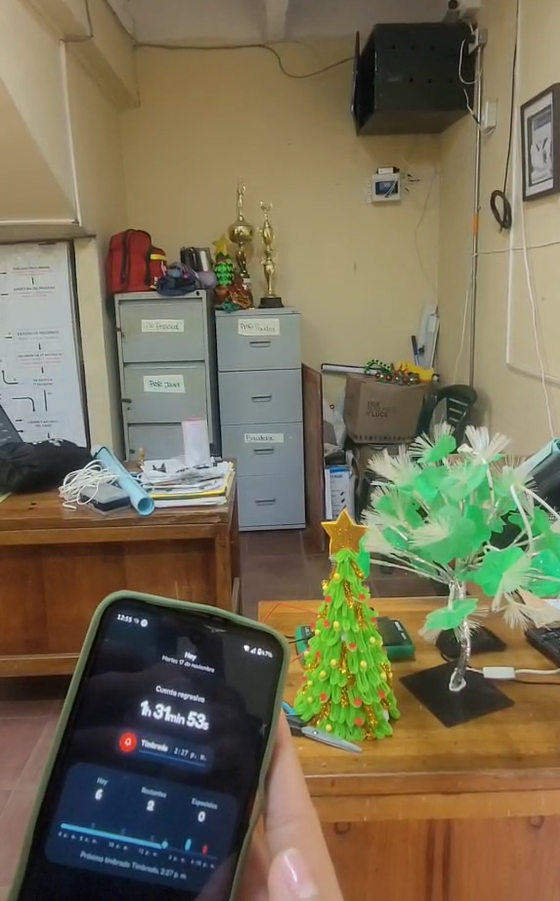
\includegraphics[width=0.88\linewidth]{figuras/sitio.png}
\end{minipage}\hfill
\begin{minipage}[c]{0.6\linewidth}
  \raggedright
  \textbf{Prueba en Cecilia de Lleras}\par\smallskip
  La foto muestra Inicio con la cuenta regresiva hacia el aviso programado de las 2:27\,p.\,m., tomada durante la espera previa. El equipo reportó que la campana tocó ese aviso en la institución \cite{informe}.
\end{minipage}
\caption{Pantalla real de Inicio durante la prueba en el sitio}
\end{figure}

\nota{\textbf{El historial no reemplaza escuchar el timbre.} Prueba que la campana dio la orden y cuánto duró, pero no que se oyó: si falta energía en la batería, el toque queda anotado aunque suene débil o no suene. En \textbf{Inicio}, \textbf{Hoy} y \textbf{Restantes} se calculan con el horario y la hora, no con el historial \cite{repo,firmware}.}

% ---------------------------------------------------------------------------
\clearpage
\section{Diagnóstico}
\label{sec:diagnostico}
Empiece siempre por la tarjeta de estado de \textbf{Campana}. Busque la situación en la tabla.

\begin{table}[H]
\centering\small
\caption{Problemas frecuentes y qué hacer}
\begin{tabularx}{\linewidth}{@{}P{3.9cm}YY@{}}
\toprule
\textbf{Situación} & \textbf{Qué revisar} & \textbf{Qué hacer} \\
\midrule
Android dice que la red SolarBell no tiene Internet. & Es normal: la campana no da Internet. & Elija seguir conectado y abra SolarBell. \\
Inicio muestra \textbf{Campana fuera de alcance} o Campana dice \textbf{Fuera de alcance}. & Que el teléfono esté en la red SolarBell o en la red del colegio, la distancia al gabinete y el interruptor del Wi-Fi. & Acérquese, conéctese a SolarBell y pulse \boton{Buscar campana}. Si la red SolarBell no aparece, la campana puede estar en ahorro: conéctese a la red del colegio. Cambie el interruptor solo con autorización (sección~\ref{sec:interruptor}). \\
La campana no se une a la red del colegio. & El mensaje rojo de la ventana (Tabla~\ref{tab:wifi}). & Corrija según el mensaje y repita desde la red SolarBell. Si persiste, avise a soporte. \\
Reloj \textbf{Sin hora}. & Fecha, hora y zona del teléfono. & Corrija el teléfono y vuelva a abrir la aplicación conectado a la campana. Mientras diga Sin hora, el horario no suena. \\
Un cambio desapareció o salió un aviso rojo. & Si la campana estaba fuera de alcance al guardar. & Recupere la conexión, revise la lista y repita el cambio. \\
El próximo aviso no es el esperado. & Hora del teléfono, día de la semana y si hay una fecha especial ese día. & Revise \textbf{Fechas}: una fecha en \textbf{Horario especial} o \textbf{Sin timbrado} reemplaza el horario habitual. \\
La pantalla muestra el toque, pero no se oye. & Si se quedó en \textbf{Encendiendo el inversor…} y si alguien escucha en el sitio. & Anote la hora y lo que mostraba la pantalla. Use el pulsador si el aviso es necesario y avise a soporte. \\
La batería no sostiene el timbre: el sonido sale débil, se corta o no sale, sobre todo tras días nublados. & Si el pulsador de pared sí suena (entonces el timbre está bien y falta energía). & No repita pruebas, porque cada toque gasta batería. Use el pulsador para los avisos importantes de la jornada y avise a soporte para revisar batería y panel. Si soporte lo indica, apague el Wi-Fi para ahorrar energía. \\
No sabe si un aviso sonó. & \textbf{Historial}: busque el nombre o filtre por el día. & Si no está, la campana no lo tocó: revise reloj, horario y fechas especiales. Si está como \textbf{Detenido} o \textbf{Cortado}, alguien lo interrumpió desde \textbf{Tocar}. \\
Suena a una hora no prevista. & \textbf{Historial} a esa hora: \textbf{Manual} indica una orden desde \textbf{Tocar}; \textbf{Programado}, un aviso del horario o de una fecha especial. & Suspenda las pruebas, anote lo ocurrido y avise a coordinación. Recuerde que cualquiera con la clave puede tocar. Si no aparece en el historial, pudo ser el pulsador de pared. \\
\bottomrule
\end{tabularx}
\end{table}

\begin{figure}[H]
\centering
\pantalla{inicio-fuera}{Inicio con «Campana fuera de alcance».}\hspace{1.2cm}
\pantalla{campana-fuera}{Campana: «Fuera de alcance, vista hace un momento».}
\caption{Cómo se ve la aplicación cuando no llega a la campana}
\end{figure}

\section{Fuentes}
\begingroup
\small
\renewcommand{\section}[2]{}
\begin{thebibliography}{9}
\setlength{\itemsep}{3pt}
\bibitem{repo} Equipo SolarBell. (2026). \textit{SolarBell}, rama \pin{main}, revisión \pin{0adeb14}. \href{https://github.com/AndresOrtizJDK/SolarBell/tree/0adeb14514f4e0b15457052f21800002322fbb43/frontend/src}{Código de las pantallas y estado de la aplicación}.
\bibitem{firmware} Equipo SolarBell. (2026). \textit{Campana SolarBell local}. \href{https://github.com/AndresOrtizJDK/SolarBell/tree/0adeb14514f4e0b15457052f21800002322fbb43/ESP32}{Documentación e implementación del firmware 0.8.0}.
\bibitem{apk} Equipo SolarBell. (2026). \textit{Aplicación Android de SolarBell}. \href{https://github.com/AndresOrtizJDK/SolarBell/tree/0adeb14514f4e0b15457052f21800002322fbb43/frontend/android}{Configuración del proyecto Android}.
\bibitem{informe} Equipo SolarBell. (2026). \textit{Informe final del Proyecto de Aula Semestral}. Universidad de Córdoba. Secciones 5.2 y 5.3.
\end{thebibliography}
\endgroup
\end{document}
